
%% CLASS MANUAL FOUND IN http://blog.poormansmath.net/latex-class-for-lecture-notes/ %%
%% CLASS AUTHOR Stefano Maggiolo %%
\documentclass[english,course]{Notes}

\title{COURSE CODE}
\subject{SUBJECT AREA}
\author{Joao Almeida-Domingues}
\email{2334590D@student.gla.ac.uk}
\speaker{LECTURER}
\date{07}{07}{1993}
\dateend{07}{07}{1994}
\place{University of Glasgow}

 %%%%% GENERAL MATHEMATICAL NOTATION SHORTCUTS %%%%%
 
\newcommand{\n}{\mathbb{N}}
\newcommand{\z}{\mathbb{Z}}
\newcommand{\q}{\mathbb{Q}}
\newcommand{\cx}{\mathbb{C}}
\newcommand{\real}{\mathbb{R}}
\newcommand{\field}{\mathbb{F}}
\newcommand{\ita}[1]{\textit{#1}}
\newcommand{\oneton}{\{1,2,3,...,n\}}
\newcommand\ef{\ita{f} }

\newcommand\inv[1]{#1^{-1}}
\newcommand\setb[1]{\{#1\}}
\newcommand\en{\ita{n }}
\renewcommand\qedsymbol{QED} %QED instead of square



%%%%%%%%%%%%%%%%PACKAGES%%%%%%%%%%%%%%%%%%%%%%%%%%%%%
%\usepackage{lipsum}  

\usepackage{amsmath,amsthm,amssymb,graphicx,mathtools} %maths
\usepackage{hyperref,framed,color,fancybox,todo,proof} %layout

\renewcommand{\abstractname}{\vspace{3\baselineskip}} %hack to remove abstract

% framed :  \begin{shaded,frame,snugshade or leftbar} \definecolor{shadecolor}{rgb}{XYZ} to change color
%fancybox: \shadowbox,ovalbox or doublebox
%\extra for Extra content layout box
%%%%%%%%%%%%%%%%%%%%%%%%%%%

%%%CLASS SHORTCUTS%%%%
%\lecture{day}{month}{year} for margin note 
%\begin{theorem} sdfsdf\end{theorem}  --> \theorem
%\begin{proposition} dfsdfs\end{proposition} --> \prop
%\begin{lemma} dsfsd \end{lemma} --> \lem
%\begin{corollary} f ffew \end{corollary}
%\begin{definition} fwewef w \end{definition} --> \defn
%\begin{example} feww e\end{example} --> \ex
%\begin{exercise} wefwe \end{exercise}
%\begin{remark} wef we \end{remark} --> \rem
%\begin{fact} wefe \end{fact}
%\begin{problem} wef ew \end{problem}
%\begin{conjecture} ewfew \end{conjecture}
%\begin{claim} few w \end{claim}
%\begin{notation} fewf \end{notation} --> \nota
%\mymarginpar for scriptsize margin

\begin{document}

\begin{abstract}
\par{These lecture notes were collated by me from a mixture of sources , the two main sources being the lecture notes provided by the lecturer and the content presented in-lecture. All other referenced material (if used) can be found in the \ita{Bibliography} and \ita{References} sections.}
\par{The primary goal of these notes is to function as a succinct but comprehensive revision aid, hence if you came by them via a search engine , please note that they're not intended to be a reflection of the quality of the materials referenced or the content lectured.}
\par{Lastly, with regards to formatting, the pdf doc was typeset in \LaTeX , using a modified version of Stefano Maggiolo's \href{http://blog.poormansmath.net/latex-class-for-lecture-notes/}{\underline{\textcolor{blue}{class}}}}
\end{abstract}

\newpage

\section{Propositional Logic}

\defn{Propositional Logic}{the logic of compound statements built from simpler statements using Boolean connectives}

\defn{Propostion}{declarative sentence which is either true or false}

\todo{See slide annotations}

\todo{Truth table for all connectives , use the succinct style, where for large statements the result is written under the connective}
\todo{Write a remark explaining the use of the succinct form of the tables for large compound propositions (e.g. (p > q) \& (~p v q) one would not make a separate column for the conjunction, but instead just write the result under the \&)}
\todo{Write a remark explaining that for any n propositions, rows = $2^{n}$, since for every p {1,0}}
%%%%%%%%%%%%%%%%%%%%%%%%%%%%%%%%%%%%%%%%%%%%%%%%%%%%%%%%%%%%%%%%%%%%%%%%
\section{}
%%%%%%%%%%%%%%%%%%%%%%%%%%%%%%%%%%%%%%%%%%%%%%%%%%%%%%%%%%%%%%%%%%%%%%%%

%%%%%%%%%%%%%%%%%%%%%%%%%%%%%%%%%%%%%%%%%%%%%%%%%%%%%%%%%%%%%%%%%%%%%%%%
\section{}
%%%%%%%%%%%%%%%%%%%%%%%%%%%%%%%%%%%%%%%%%%%%%%%%%%%%%%%%%%%%%%%%%%%%%%%%

%%%%%%%%%%%%%%%%%%%%%%%%%%%%%%%%%%%%%%%%%%%%%%%%%%%%%%%%%%%%%%%%%%%%%%%%
\section{}
%%%%%%%%%%%%%%%%%%%%%%%%%%%%%%%%%%%%%%%%%%%%%%%%%%%%%%%%%%%%%%%%%%%%%%%%

%%%%%%%%%%%%%%%%%%%%%%%%%%%%%%%%%%%%%%%%%%%%%%%%%%%%%%%%%%%%%%%%%%%%%%%%
\section{Proofs}
%%%%%%%%%%%%%%%%%%%%%%%%%%%%%%%%%%%%%%%%%%%%%%%%%%%%%%%%%%%%%%%%%%%%%%%%

\subsection{Rules of Inference}

\defn{Valid Argument}{the truth of the premises logically guarantees the truth of the conclusion , \ita{i.e.} $(p \land q \land r \land \dots) \rightarrow q$ is a tautology}

\mymarginpar{Memorising not required}

\subsubsection{Modus Ponens}
\begin{minipage}{.5\textwidth}
\infer{q}{p & (p \rightarrow q)}
\end{minipage}
\begin{minipage}{.5\textwidth}
\centering
\begin{tabular}{@{ }c@{ }@{ }c | c@{ }@{}c@{}@{ }c@{ }@{ }c@{ }@{}c@{}@{ }c@{ }@{ }c@{ }@{ }c@{ }@{}c@{}@{}c@{}@{ }c@{ }@{ }c@{ }@{ }c}
$p$ & $q$ &  & ( & $p$ & $\land$ & ( & $p$ & $\rightarrow$ & $q$ & ) & ) & $\rightarrow$ & $q$ & \\
\hline 
1 & 1 &  &  & 1 & 1 &  & 1 & 1 & 1 &  &  & \textcolor{red}{1} & 1 & \\
1 & 0 &  &  & 1 & 0 &  & 1 & 0 & 0 &  &  & \textcolor{red}{1} & 0 & \\
0 & 1 &  &  & 0 & 0 &  & 0 & 1 & 1 &  &  & \textcolor{red}{1} & 1 & \\
0 & 0 &  &  & 0 & 0 &  & 0 & 1 & 0 &  &  & \textcolor{red}{1} & 0 & \\
\end{tabular}
\end{minipage}


\subsubsection{Modus Tolens}

\begin{minipage}{.5\textwidth}
\infer{\lnot q}{\lnot q & (p \rightarrow q)}
\end{minipage}
\begin{minipage}{.5\textwidth}
\centering
\begin{tabular}{@{ }c@{ }@{ }c | c@{ }@{}c@{}@{ }c@{ }@{ }c@{ }@{ }c@{ }@{}c@{}@{ }c@{ }@{ }c@{ }@{ }c@{ }@{}c@{}@{}c@{}@{ }c@{ }@{ }c@{ }@{ }c@{ }@{ }c}
$p$ & $q$ &  & ( & $\lnot$ & $q$ & $\land$ & ( & $p$ & $\rightarrow$ & $q$ & ) & ) & $\rightarrow$ & $\lnot$ & $p$ & \\
\hline 
1 & 1 &  &  & 0 & 1 & 0 &  & 1 & 1 & 1 &  &  & \textcolor{red}{1} & 0 & 1 & \\
1 & 0 &  &  & 1 & 0 & 0 &  & 1 & 0 & 0 &  &  & \textcolor{red}{1} & 0 & 1 & \\
0 & 1 &  &  & 0 & 1 & 0 &  & 0 & 1 & 1 &  &  & \textcolor{red}{1} & 1 & 0 & \\
0 & 0 &  &  & 1 & 0 & 1 &  & 0 & 1 & 0 &  &  & \textcolor{red}{1} & 1 & 0 & \\
\end{tabular}
\end{minipage}

\todo{Tautology truth tables}

\subsubsection{Hypothetical Syllogism}

\begin{minipage}{.5\textwidth}
\infer{p \rightarrow r}{(p \rightarrow q) & (q \rightarrow r)}
\end{minipage}

\subsubsection{Disjunctive Syllogism}

\begin{minipage}{.5\textwidth}
\infer{q}{p \lor q & \lnot p}
\end{minipage}

\subsubsection{Resolution}

\begin{minipage}{.5\textwidth}
\infer{q \lor r}{p \lor q & \lnot p \lor r}
\end{minipage}

\subsubsection{Addition}

\begin{minipage}{.5\textwidth}
\infer{p \lor q}{p}
\end{minipage}

\subsubsection{Simplification}

\begin{minipage}{.5\textwidth}
\infer{p}{p \land q}
\end{minipage}

\subsubsection{Conjunction}

\begin{minipage}{.5\textwidth}
\infer{p \land q}{p & q}
\end{minipage}

\todo{Example slides 26,27}

\subsection{Constructing a Proof Tree}

\par{Continuing with the example above, we can construct a \ita{proof tree}, where each \ita{leaf} is composed of axioms - the premises, and the conclusion sits at the \ita{root}}

\todo{slide 33}

\subsection{Quantifiers}



\newpage

\section{Induction and Recursive Definitions}

\defn{Kleene Star}{is a unary operation on strings or , more generally , sets of symbols}

\nota{$V^{\ast}$ , where $V$ is the set being operated on}


\newpage

\section{Graphs}

\par{See 2P notes \url{https://github.com/Joe-a-d/LectureNotesUniversityOfGlasgow/tree/master/Year2/Graphs\&Networks/2P.pdf}}

\begin{itemize}
	\item Fundamentals
	\item Isomorphism
	\item Eulerian 
	\item Hamiltonian
\end{itemize}

\example{ How many simple undirected graphs are there with 20 vertices and 60 edges? \\

\par{For every pairs of vertices one has a possible edge, hence $K_{20}$ has ${20\choose2} = 190$ edges  For a  graph  to  have  $60$  edges  we  need  to  choose  $60$  out  of  $190$  possible  edges.  The number of graphs therefore equals ${190\choose60} = \frac{190!}{60!30!}
$}
}
\section{Relations}

\defn{Binary Relation}{for two sets $A , B$ , $R \subseteq A \times B$ , where each element of $R$ is the set of related ordered pairs $(a,b) $ for $a \in A , b \in B$  . We say that \ita{``a is related to b by $R$''}}

\par{We can also represent relations as graphs, where the nodes are the individual elements of $A,B$ present in $R$, and its edges are the ordered pairs}

\example{Take $A = 1,2,3,4$ and $R = a | b $ for $a , b \in A $. In this case $R$ operates over the same set, hence $R \subseteq A \times A$. Now let $G(V,E)$ be the graph representing this relation then :

$$V = \{1,2,3,4\} \text{   and   } E=\{(1,1),(1,2),(1,3),(1,4),(2,2),(2,4),(3,3),(4,4) $$

\IfFileExists{relationGraph.png}{}{\write18{wget https://cdn.mathpix.com/snip/images/kjGI8Fl8m-lGFWL8E0dg77jv7-AN1UAEKTuinYhTPEI.original.fullsize.png -O relationGraph.png}}
\begin{figure}[ht]
\centering
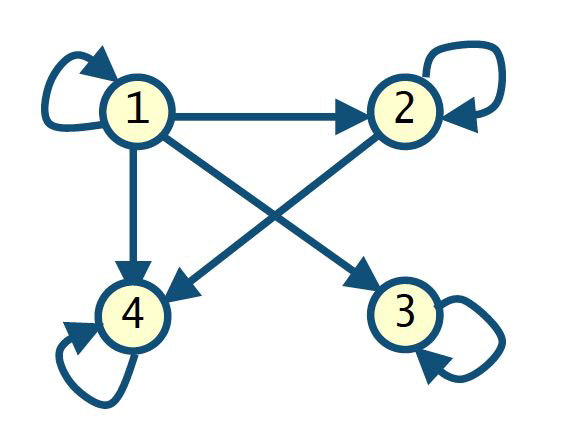
\includegraphics[width=0.5\textwidth]{relationGraph.png}
\end{figure}

\rem{Relations are not exclusively binary , for a relation between $n$ sets we have a set $R$ of $n-$tupples}

\subsection{Properties}

\begin{itemize}
	\item[] Reflexive : $a \in A \implies (a,a) \in R $
	\item[] Symmetric $a , b \in A , a \neq b \text{ and } (a,b) \in R \implies (b,a) \in R$
	\item[] Anti-Symmetric $a , b \in A , a \neq b \text{ and } (a,b) \in R \implies (b,a) \not\in R$
	\item[] Transitive $a , b , c \in A , a \neq b \neq c \; (a,b) , (b,c) \in R \implies (a,c) \in R$
\end{itemize}

\defn{Equivalence Relation}{$R$ is an equivalence relation \ita{iff} it is reflexive, symmetric and transitive}

\example{Take $(a,b) \in R \iff ``a$ is strictly taller than $b$'' , i.e $\mathop{height}(a) > \mathop{height}(b)$  . Then, (1) $R$ is not reflexive, since $\mathop{height}(a) = \mathop{height}(a)$ (2) $R$ is not symmetric given that $b$ is strictly smaller (not taller) than $a$ , $\mathop{height}(b) < \mathop{height}(a)$ (3) $R$ is anti-symmetric since, $\mathop{height}(b) < \mathop{height}(a)$. Finally (4) $R$ is transitive since if $a$ is taller than $b$ and $b$ is taller than $c$ then $a$ is taller than $c$}



\todo{add bib: Truth Tables : Michael Rieppel ``mrieppel '' @https://github.com/mrieppel/TruthTableGenerator}

\todos

\end{document}